\clearpage
\section{Phase portrait of the conservative pendulum}
I'll define a helper variable 
\begin{equation}
    v = \dot{\theta}
\end{equation}
so the equation becomes 
\begin{equation}
    \dot{v}=-\sin\theta
\end{equation}
\subsection{fixed points}
at the fixed points 
\begin{equation}
    v=0,\quad \sin\theta=0
\end{equation}
so 
\begin{equation}
    \ins{\theta^*,v^*}=\ins{\pi n,0}
\end{equation}
next the jacobian is 
\begin{equation}
    J = \mqty(0&1\\-\cos\theta&0)
\end{equation}
we can split the fixed points into two groups, for even and odd \(n\). Even \(n\) gives \(\cos(\cdots)=1\) therefore the eigenvalues are \(\pm i\), so these are linear centers. Odd \(n\) gives \(\cos(\cdots)=-1\) so the eigenvalues are \(\pm 1\), and since both eigenvalues are real but one is positive and the other is negative these are saddles.
\subsection{genuine centers}
Conservation of energy guarantees this. This can be shown explicitly by calculating the energy, but even a verbal argument I believe shows this. If we assume a trajectory which either spirals into or away from one such fixed point, it means the pendulum must be simultaneously moving away/toward from the fixed point physically and also gathering/losing velocity as it does so. This means energy is introduced/taken away from the system. Since this is impossible as we assume an isolated system, trajectories must be closed curves surrounding the fixed points, meaning they are genuine centers.
\subsection{phase plane}
\begin{figure}[H]
    \centering
    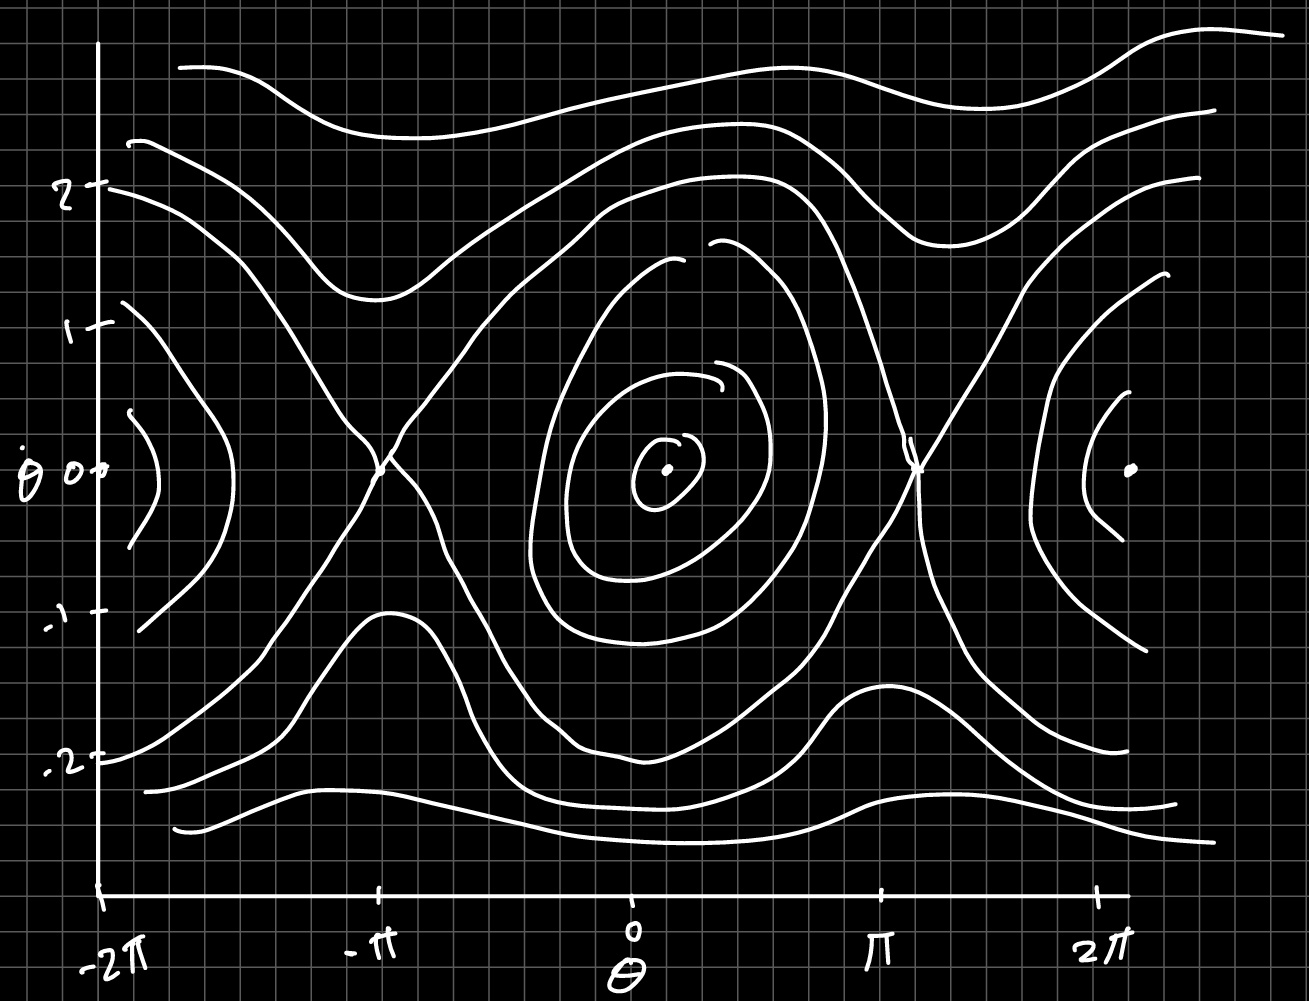
\includegraphics[width=0.75\textwidth]{fig3.png}
\end{figure}
The energy of the system is 
\begin{equation}
    E = \frac{1}{2}v^2+1-\cos\theta
\end{equation}
and the energy at the saddle points is 
\begin{equation}
    E((2m+1)\pi,0)=1-\cos\ins{\ins{2m+1}\pi}=2
\end{equation}
so the separatrix is 
\begin{equation}
    \frac{1}{2}v^2+1-\cos\theta=2
\end{equation}
solving for v 
\begin{equation}
    v = \pm\sqrt{2\ins{1+\cos\theta}}
\end{equation}
which can be written as 
\begin{equation}
    v = \pm2 \cos\ins{\frac{\theta}{2}}
\end{equation}
which represents a pendulum with just enough energy to reach the top of its motion with 0 velocity.